
\documentclass[10pt,a4paper]{article}
\usepackage[T1]{fontenc}
\usepackage{tikz}
\usepackage[margin=1cm]{geometry}
\begin{document}

\section*{Step-by-Step Tree Construction}
This document provides a step-by-step view of the binary search tree (BST) construction process. Each step illustrates the tree's state after a new node is inserted.

\subsection*{Algorithm for Tree Construction}
The binary search tree was constructed using the following steps:
\begin{enumerate}
    \item \textbf{Empty Tree Initialization:} Begin with an empty tree.
    \item \textbf{Node Insertion:} For each node insertion:
    \begin{itemize}
        \item Start at the root and compare the new node's value with the current node.
        \item Move left if the new value is smaller, or right if it is larger.
        \item Insert the new node into the first available position that maintains the BST property.
    \end{itemize}
    \item \textbf{Recursive Traversal:} Insert nodes recursively to ensure that each node's left subtree contains values less than the node and the right subtree contains values greater.
\end{enumerate}

\subsection*{Step-by-Step Visualization}
The following figures show the BST after each insertion step. Each step highlights the newly added node in pink to indicate the changes made.


\begin{figure}[h!]
\centering

\begin{minipage}{0.8\textwidth}
    \centering
    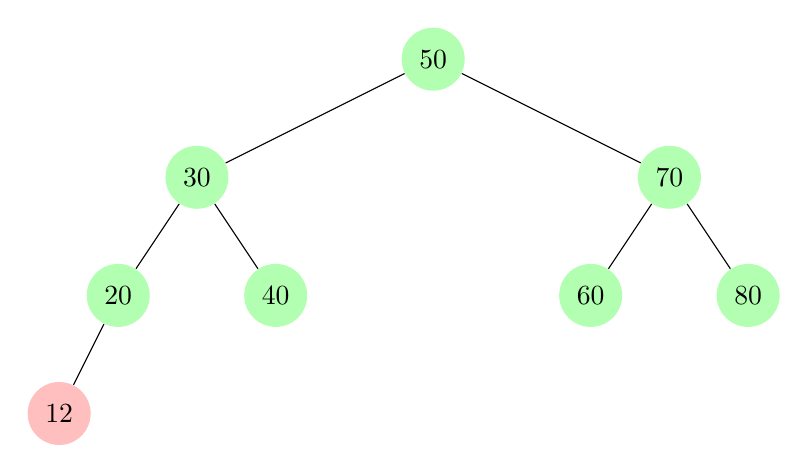
\begin{tikzpicture}[level distance=15mm, sibling distance=20mm]
        \tikzstyle{every node}=[circle,inner sep=1pt, minimum size=8mm]
        \tikzstyle{level 1}=[sibling distance=60mm, set style={{every node}+=[fill=green!30]}]
        \tikzstyle{level 2}=[sibling distance=20mm, set style={{every node}+=[fill=green!30]}]
        \tikzstyle{level 3}=[sibling distance=15mm, set style={{every node}+=[fill=green!30]}]
        \tikzstyle{level 4}=[sibling distance=10mm, set style={{every node}+=[fill=green!30]}]
        \node [fill=green!30] {50} child {node [fill=green!30] {30} child {node [fill=green!30] {20} child {node [fill=pink] {12} } child[fill=none] {edge from parent[draw=none]}} child {node [fill=green!30] {40} }} child {node [fill=green!30] {70} child {node [fill=green!30] {60} } child {node [fill=green!30] {80} }};
    \end{tikzpicture}
    \caption{Step 1}
\end{minipage}
\vspace{1cm}

\begin{minipage}{0.8\textwidth}
    \centering
    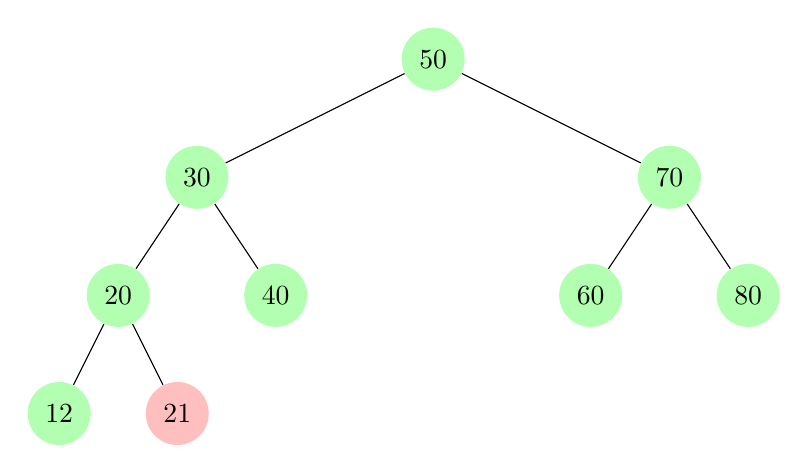
\begin{tikzpicture}[level distance=15mm, sibling distance=20mm]
        \tikzstyle{every node}=[circle,inner sep=1pt, minimum size=8mm]
        \tikzstyle{level 1}=[sibling distance=60mm, set style={{every node}+=[fill=green!30]}]
        \tikzstyle{level 2}=[sibling distance=20mm, set style={{every node}+=[fill=green!30]}]
        \tikzstyle{level 3}=[sibling distance=15mm, set style={{every node}+=[fill=green!30]}]
        \tikzstyle{level 4}=[sibling distance=10mm, set style={{every node}+=[fill=green!30]}]
        \node [fill=green!30] {50} child {node [fill=green!30] {30} child {node [fill=green!30] {20} child {node [fill=green!30] {12} } child {node [fill=pink] {21} }} child {node [fill=green!30] {40} }} child {node [fill=green!30] {70} child {node [fill=green!30] {60} } child {node [fill=green!30] {80} }};
    \end{tikzpicture}
    \caption{Step 2}
\end{minipage}
\vspace{1cm}

\begin{minipage}{0.8\textwidth}
    \centering
    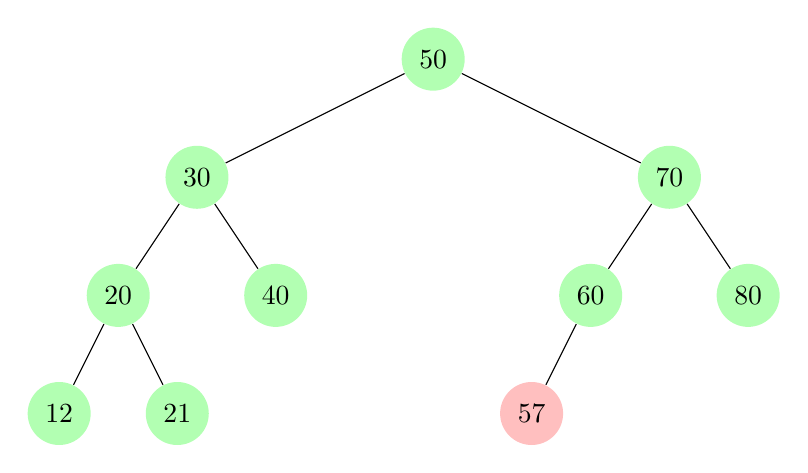
\begin{tikzpicture}[level distance=15mm, sibling distance=20mm]
        \tikzstyle{every node}=[circle,inner sep=1pt, minimum size=8mm]
        \tikzstyle{level 1}=[sibling distance=60mm, set style={{every node}+=[fill=green!30]}]
        \tikzstyle{level 2}=[sibling distance=20mm, set style={{every node}+=[fill=green!30]}]
        \tikzstyle{level 3}=[sibling distance=15mm, set style={{every node}+=[fill=green!30]}]
        \tikzstyle{level 4}=[sibling distance=10mm, set style={{every node}+=[fill=green!30]}]
        \node [fill=green!30] {50} child {node [fill=green!30] {30} child {node [fill=green!30] {20} child {node [fill=green!30] {12} } child {node [fill=green!30] {21} }} child {node [fill=green!30] {40} }} child {node [fill=green!30] {70} child {node [fill=green!30] {60} child {node [fill=pink] {57} } child[fill=none] {edge from parent[draw=none]}} child {node [fill=green!30] {80} }};
    \end{tikzpicture}
    \caption{Step 3}
\end{minipage}
\vspace{1cm}

\end{figure}
\newpage

\begin{figure}[h!]
\centering

\begin{minipage}{0.8\textwidth}
    \centering
    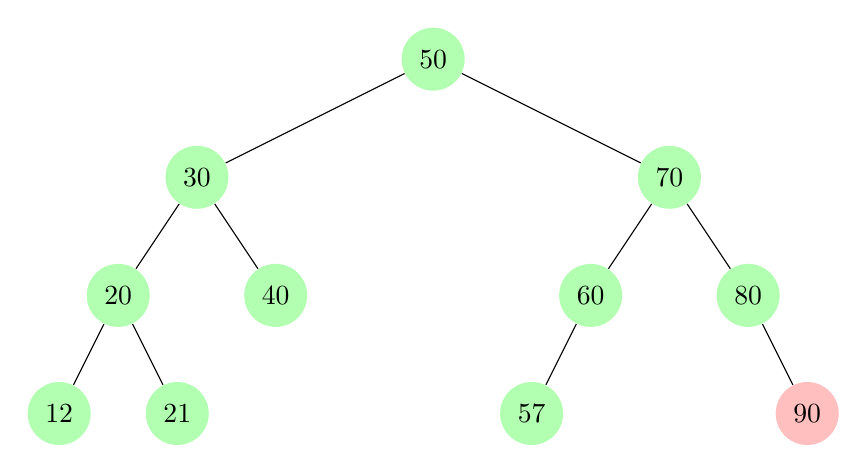
\begin{tikzpicture}[level distance=15mm, sibling distance=20mm]
        \tikzstyle{every node}=[circle,inner sep=1pt, minimum size=8mm]
        \tikzstyle{level 1}=[sibling distance=60mm, set style={{every node}+=[fill=green!30]}]
        \tikzstyle{level 2}=[sibling distance=20mm, set style={{every node}+=[fill=green!30]}]
        \tikzstyle{level 3}=[sibling distance=15mm, set style={{every node}+=[fill=green!30]}]
        \tikzstyle{level 4}=[sibling distance=10mm, set style={{every node}+=[fill=green!30]}]
        \node [fill=green!30] {50} child {node [fill=green!30] {30} child {node [fill=green!30] {20} child {node [fill=green!30] {12} } child {node [fill=green!30] {21} }} child {node [fill=green!30] {40} }} child {node [fill=green!30] {70} child {node [fill=green!30] {60} child {node [fill=green!30] {57} } child[fill=none] {edge from parent[draw=none]}} child {node [fill=green!30] {80} child[fill=none] {edge from parent[draw=none]} child {node [fill=pink] {90} }}};
    \end{tikzpicture}
    \caption{Step 4}
\end{minipage}
\vspace{1cm}

\end{figure}
\newpage

\end{document}
